\documentclass[12pt, oneside]{article}
\usepackage[letterpaper, margin=1in, headsep=0.5in, left=0.3in, right=2.5in]{geometry}
\usepackage[english]{babel}
\usepackage[utf8]{inputenc}
\usepackage{amsmath}
\usepackage{amsfonts}
\usepackage{amssymb}
\usepackage{tikz}
\usepackage{yhmath}
\usetikzlibrary{quotes, angles}
\usepackage{graphicx}
\usepackage{enumitem}
\usepackage{multicol}

\newif\ifmeta
\metatrue %print standards and topics tags

\title{Regents Geometry}
\author{Chris Huson}
\date{May 2022}

\usepackage{fancyhdr}
\pagestyle{fancy}
\fancyhf{}
\renewcommand{\headrulewidth}{0pt} % disable the underline of the header
\raggedbottom

%\fancyhead[LE]{\thepage}
\fancyhead[RO]{Name:}
\fancyhead[LO]{BECA / Dr. Huson / Geometry Regents Mixed Review}
\cfoot{\thepage}

\begin{document}
\subsubsection*{11.14 Triangle dilation}
\begin{enumerate}[itemsep=1.2cm]
    \item Triangle $ABC$ is dilated with a scale factor of $k$ centered at $A$, yielding $\triangle ADE$, as shown. Given $AB=9$, $BD=3$, $AC=10$, and $DE=12$. Find $BC$.
    \begin{center}
      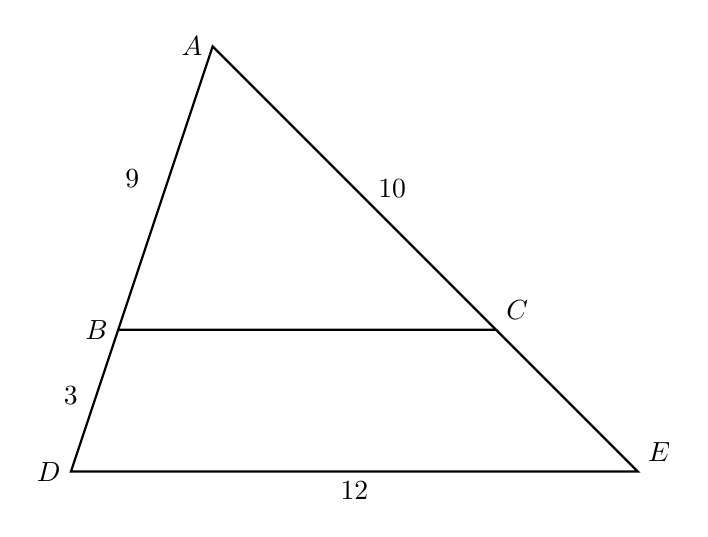
\begin{tikzpicture}[scale=0.6]
        \draw [thick]
        (0,0)node[left]{$B$}--
        (8,0)node[above right]{$C$}--
        (2,6)node[left]{$A$}--cycle;
        \draw [thick]
        (0,0)--
        (-1,-3)node[left]{$D$}--
        (11,-3)node[above right]{$E$}--(8,0);
        \node at (-1,-1)[below]{$3$};
        \node at (5.3, 3)[right]{$10$};
        \node at (0.3, 2.8)[above]{$9$};
        \node at (5,-3)[below]{$12$};
      \end{tikzpicture}
    \end{center}

\item What is an equation of the line that passes through the point $(-2,5)$ and is perpendicular to a line with equation $y=\frac{3}{4}x+5$?
    \begin{multicols}{2}
    \begin{enumerate}
        \item $y-2=\frac{4}{3}(x+5)$
        \item $y-2=-\frac{4}{3}(x+5)$ 
        \item $y+2=\frac{4}{3}(x-5)$
        \item $y+2=-\frac{4}{3}(x-5)$
    \end{enumerate}
    \end{multicols}


\item A beach tent can be modeled as a pyramid with a square base whose sides measure 72 inches and whose height measures 96 inches. What is the volume of the tent, to the \emph{nearest cubic foot}?

\item The equation of a cirle is $x^2+y^2-12x-2y=27$. What are the center and radius of the circle?

\item Point $M$ divides $\overline{AB}$ so that $AM:MB = 1:4$. If $A$ has coordinates $(1,-1)$ and $B$ has coordinates $(6,9)$, what are the coordinates of $M$?

\newpage
\item From three miles away, the angle of elevation to the top of a radio tower is $4.0^\circ$. What is the height of the tower, to the \emph{nearest ten feet}? (1 mile = 5280 feet)
  \begin{center}
    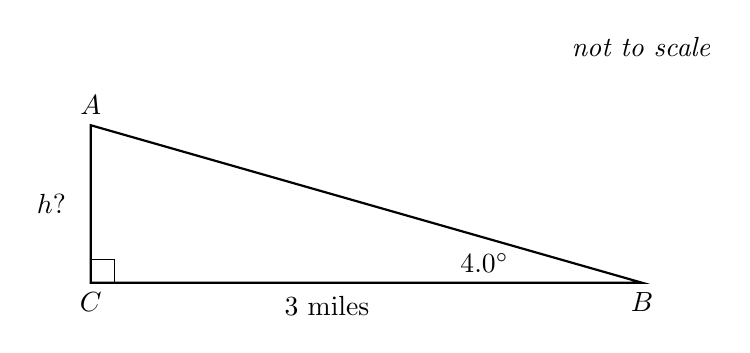
\begin{tikzpicture}[scale=1]
    \draw [thick]
      (0,0)node[below]{$B$}--
      (-7,2)node[above]{$A$}--
      (-7,0)node[below]{$C$}--cycle;
      \draw (-7,0)++(0.3,0)--++(0,0.3)--+(-0.3,0);
      \node at (-7.5,1){$h?$};
      \node at (-2,0.25){$4.0^\circ$};
      \node at (-4,-0.3){3 miles};
      \node at (0,3){\emph{not to scale}};
  \end{tikzpicture}
  \end{center}

\item If a circular disk is continuously rotated around its diameter, what is the three-dimensional figure formed?
  \begin{multicols}{2}
  \begin{enumerate}
    \item cone
    \item sphere
    \item cylinder
    \item rectangular prism
  \end{enumerate}
\end{multicols}

\item Given right triangle $ABC$ with a right angle at $C$, $m\angle A=33^\circ$. Given right triangle $XYZ$ with a right angle at $Z$, $m\angle Y=57^\circ$.
  \begin{center}
    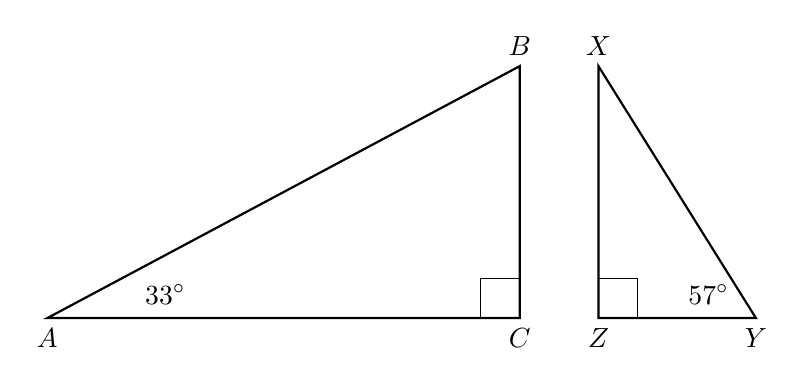
\begin{tikzpicture}[scale=1]
    \draw [thick]
      (0,0)node[below]{$Z$}--
      (2,0)node[below]{$Y$}--
      (0,3.2)node[above]{$X$}--cycle;
      \draw (0,0)++(0.5,0)--++(0,0.5)--+(-0.5,0);
    \draw [thick]
      (-7,0)node[below]{$A$}--
      (-1,3.2)node[above]{$B$}--
      (-1,0)node[below]{$C$}--cycle;
      \draw (-1,0)++(-0.5,0)--++(0,0.5)--+(0.5,0);
      \node at (-5.5,0.3){$33^\circ$};
      \node at (1.4,0.3){$57^\circ$};
  \end{tikzpicture}
  \end{center}
Which proportion in relation to $\triangle ABC$ and $\triangle XYZ$ is \emph{not} correct?
  \begin{multicols}{2}
    \begin{enumerate}
      \item $\displaystyle \frac{AC}{AB} = \frac{XZ}{XY}$
      \item $\displaystyle \frac{BC}{AC} = \frac{YZ}{XZ}$ 
      \item $\displaystyle \frac{AC}{XZ} = \frac{BC}{YZ}$
      \item $\displaystyle \frac{BC}{XZ} = \frac{AB}{XY}$
    \end{enumerate}
  \end{multicols}

\end{enumerate}
\end{document}
  